\documentclass[conference]{IEEEtran}
\IEEEoverridecommandlockouts
% The preceding line is only needed to identify funding in the first footnote. If that is unneeded, please comment it out.
\usepackage{cite}
\usepackage{amsmath,amssymb,amsfonts}
\usepackage{algorithmic}
\usepackage{graphicx}
\usepackage{textcomp}
\usepackage{xcolor}
\usepackage{calc}
\usepackage{cclicenses}
\usepackage{enumitem}
\setlist[description]{nosep, topsep = 1em, labelindent=0em, listparindent=4em, leftmargin=1em}%


\def\BibTeX{{\rm B\kern-.05em{\sc i\kern-.025em b}\kern-.08em
    T\kern-.1667em\lower.7ex\hbox{E}\kern-.125emX}}

\makeatletter
\def\ps@IEEEtitlepagestyle{%
	\def\@oddfoot{\mycopyrightnotice}%
	\def\@evenfoot{}%
}
\def\mycopyrightnotice{%
	{\footnotesize \copyright Alain Brenzikofer\hfill\hfill encointer.org\hfill first published on 18.11.2018, preliminary V0.13, 09.12.2020}% <--- Change here
	\gdef\mycopyrightnotice{}% just in case
}

\newcommand{\executeiffilenewer}[3]{%
	\ifnum\pdfstrcmp{\pdffilemoddate{#1}}%
	{\pdffilemoddate{#2}}>0%
	{\immediate\write18{#3}}\fi%
}
\newcommand{\includesvg}[1]{%
	\executeiffilenewer{#1.svg}{#1.pdf}%
	{inkscape -z -D --file=#1.svg %
		--export-pdf=#1.pdf --export-latex}%
	\input{#1.pdf_tex}%
}

\newtheorem{erule}{Rule}
\newtheorem{hypothesis}{Hypothesis}
%\usepackage{draftwatermark}
\begin{document}
%\SetWatermarkText{Confidential Draft}
%\SetWatermarkScale{0.5}
\newcommand{\encointer}{\textsl{encointer} }



\title{\encointer - An Ecological, Egalitarian and Private Cryptocurrency and Digital Personhood System\\
%\thanks{Identify applicable funding agency here. If none, delete this.}
}

\author{\IEEEauthorblockN{Alain Brenzikofer}
%\IEEEauthorblockA{\textit{dept. name of organization (of Aff.)} \\
%\textit{name of organization (of Aff.)}\\
%City, Country \\
alain@encointer.org}
%\and
%\IEEEauthorblockN{2\textsuperscript{nd} Given Name Surname}
%\IEEEauthorblockA{\textit{dept. name of organization (of Aff.)} \\
%\textit{name of organization (of Aff.)}\\
%City, Country \\
%email address}

\maketitle


\begin{abstract}
\encointer proposes a new blockchain based cryptocurrency with  an egalitarian money supply policy. Money issuance is done through a universal basic income subject to a proof-of-personhood. Only individuals attending randomized pseudonym key signing events obtain such proofs. \encointer also features private transactions and scalable, trustless off-chain smart contracts enabled by trust3ed execution environments.
\end{abstract}

\begin{IEEEkeywords}
cryptocurrency, macroeconomics, identity management, location awareness, privacy, energy efficiency, digital personhood
\end{IEEEkeywords}

\section{Motivation}
\subsection{Economics}
With the appearance of Bitcoin \cite{nakamoto08} in 2008, a big socio-economic experiment took off. The nature of money itself was widely debated. Bitcoin adopts a hard-coded nominally inflatonary monetary policy saturating at a fixed supply. Rapid adoption made Bitcoin a real deflationary currency, which it will remain if successful. Early adopters made a fortune. Because of its deflationary nature, bitcoin favors accumulation of capital for the few. Wealth increases without work.

The monetary policy followed by central banks issuing national fiat money on the other hand often follows the goal of price stability, aiming at a moderate inflation goal in the order of 1-2\%. Issuance of money is appointed to banks who give credit to companies who employ workers who consume goods and thereby make companies profitable and raise the GDP. A process that allegedly benefits everyone. 
However, the observation that an increase in money supply doesn't benefit everyone equally is referred to as the Cantillon-Effect \cite{cantillon}. Thomas Piketty shows \cite{piketty} that gains on capital historically exceed economic growth, another factor that questions the trickle-down theory. 

\encointer aims at turning this logic upside-down and lets all individuals issue money subject to common rules. In order to mint \encointer, people need to attend to pseudonym key signing parties (meetups) that happen at regular intervals at high sun all over the world within small randomized groups of people. The \encointer issuance therefore represents a form of \textit{universal basic income} (UBI) for every person attending such meetups. 

These \encointer meetups are at the same time the basis of a self-sovereign identity claim called proof-of-personhood (PoP) \cite{ford08} \cite{pop}, proving a one-to-one relationship between a person and her digital identity. One person can only maintain one individuality claim because ceremonies are designed to make it impossible to attend two meetups physically as they happen in different places concurrently. 
%\encointer PoP supports the standard for decentralized self-sovereign identity defined in \cite{ssi}.

\subsection{Unpermissioned Consensus}
Bitcoin and many other cryptocurrencies use an energy-hungry consensus mechanism called proof of work (PoW). While PoW has been the key idea that made Bitcoin possible in the first place, it is not ecologically sustainable. Moreover, it failed its goal of decentralization as mining has become centralized by a single company in a single country. 

Peercoin \cite{sunnyking12} introduced the first proof-of-stake (PoS) cryptocurrency in 2012. Until today, PoS is not academically respected as a sound consensus mechanism \cite{poelstra15}. While PoW makes a compromise on energy efficiency, PoS makes the compromise of benefitting the rent-seeking wealthy.

Accepting that there's always a compromise to make, \encointer introduces dPoET; a permissionless version of proof-of-elapsed-time (PoET) \cite{poet}, relying on trusted execution environments (TEE). PoET requires trust in vendor attestation services. Currently, there are few TEE vendors on the market (i.e. Intel SGX \cite{costan16}, ARM trust zone \cite{trustzone} used by AMD, Qualcomm and others) but there are also open-source hardware initiatives that might one day diversify the attestation trust. 

\subsection{Private Smart Contracts}
In 2015 Ethereum \cite{ethereum} was introduced, bringing turing-complete smart contracts to the blockchain. Ethereum now serves as a platform for many decentralized applications (DApps) and has become the major ecosystem for ICOs. While enabling publicly verifyable smart contracts, there is no way to process private data on Ethereum in trustless manner. Public unpermissioned validation of smart contracts is only possible with a minimum of public inputs. Support for zk-SNARKS has been added to the etheremun virtual machine with the metropolis hard-fork, yet this only enables to verify zero knowledge proofs that have been generated off-chain. It is therefore possible to hide the payload of a smart contract call, but as you have to call the contract by means of a public transaction, your pseudonym is leaking. Quorum \cite{quorum}, an Ethereum fork, approaches privacy by delegating smart contract validation to a small group of permissioned validators using a BFT consensus and allowing Zcash-style shielded transactions to hide your pseudonym when calling a private smart contract. Such setups do not allow GDPR-compliant DApps \cite{gdpr}, \cite{gdprbc}. The reasoning is the following: In order for the DApp to comply with GDPR, the Dapp has to be run by a single operator having users opting into his privacy terms. The operator would then have to run all private contract validators by himself. Such centralization would render the use of blockchain meaningless.

\encointer enables private, decentralized DApps. As the internal state of a TEE is not leaking, they offer a way to run smart contracts with private, encrypted inputs while still offering verifyability. This has been demonstrated by Hyperledger Sawtooth Private Data Objects (PDO) \cite{sawtoothpdo}. PDOs allow to take state and execution of smart contracts off chain, thereby also improving scalability as compared to Ethereum.

\subsection{Transaction Privacy}
Bitcoin transactions are pseudonymous but not anonymous. It has been shown that identities of transacting parties can be revealed \cite{reid12}. Aiming at transaction privacy, Monero was introduced in 2014, employing the CryptoNote protocol \cite{saberhagen14}. Receiving funds in Monero means scanning every block for transactions to oneself. This task can only be taken out by full nodes as delegating it would leak private information. 
%In 2018, the protocol was improved by using Bulletproofs \cite{buenz18}. \encointer transactions are based this improved CryptoNote protocol.

Zcash was introduced in 2016 empoying the Zerocash protocol \cite{bensasson14} using zk-SNARKS to hide sender, receiver and value from third parties. Generating SNARKS to send funds is a computationally heavy process, limiting its usability for mobile and IoT devices.

For both Monero and ZCash, privacy comes at the price of large transaction size, letting the blockchain grow quickly.
Being equipped with private smart contracts, \encointer only stores tx hashes on-chain. 
 
\subsection{Scalability}
Because of its block size limit, Bitcoin can only reach about 4-7 transactions per second onchain. 
%Ethereum doesn't have such a hard cap and so far peaked at 15 tx/s.
In order to tackle Bitcoin's scalability issues, Lightning Network payment channels \cite{poon15} were introduced in 2015 and demonstrated in 2017. Scalability is achieved by bilaterally treating transactions off-chain with the option to settle the last balance at any time on-chain. Teechan \cite{lind17} was introduced in 2017, implementing payment channels in TEEs. 

% TODO: direct invocation SubstraTEE
\encointer takes transactions and smart contract execution off-chain altogether. Only one hash per transaction must be stored onchain. The latest state is shared among validators but only the hash of that state needs to be onchain. This improves scalability by an order of magnitude and delays the need for second layer solutions. 
%As TEEs have limited memory resources, there will
%If needed, a solution similar to Teechan would fit well into the \encointer concept as a payment channel solution.

\subsection{Governance}
Decentralized blockchain governance has in the past been tried by various means. In the case of Bitcoin, a balance of power between miners and coin holders decides about the future of the protocol, which lead to multiple chain forks in the past, hurting the ecosystem and dividing development teams. 

PoS blockchains delegate governance to their whales. Who has more coin has more say. This poses a conflict of interest i.e. in the case of deciding the future nominal inflation. 

As \encointer has an anti-sybil attack measure in place (uPoP), a one-person-one-vote (1p1v) scheme can be implemented within the boundaries of one local currency community. Deciding on the parameters of a local currency should be left to the community maintaining and using it.

Global protocol decisions can't simply be delegated to all persons from all local currency communities because the trust model doesn't reach beyond the currency that you yourself participate in (attackers can undetectably build bot communities as long as they never interact with honest humans). 

One way to extend the trust model are decentralized exchanges among \encointer currencies. Communities that buy each other's coins obviously trust the integrity of the other community. Even more trust comes from people traveling and are participating in different communities. If there is one community that acts as a root of trust, a global 1p1v scheme becomes possible.

\encointer appoints a root of limited trust to a Swiss association holding the \encointer trademark. 
The association defines and audits the root-of-trust community and suggests protocol updates in advance, including changes of rewards and fees or block size limits. Suggestions by the association can be blocked by a referendum vote requiring a majority of 2/3 of voters. Balloting happens on-chain anonymously. The 2/3 majority threshold for referendums allows the association to react quickly to changing circumstances but still provide decentralization, given large opposition.

If the \encointer association should fail to suggest necessary changes, the community may suggest changes as well. They also require a majority of 2/3 of stake and 2/3 majority of 1p1v voters.

\section{Local Currencies}
Encointer has no single currency. It manages an unpermissioned set of many local currencies. Every geographically bound community can have their own local currency.

\subsection{Bootstrapping a Local Currency}
Initiators of a new local \encointer currency need to define its geographical bound by a large set $L_C$ of possible publicly accessible meetup locations $l_{C,q}$ as shown in figure \ref{fig:map}. As people will have to attend some meetup at a random location from the set $L_C$, the geographical extension should be chosen reasonably such that people only need to travel within acceptable ranges. In order to improve meetup randomization, the set of possible meetup locations should be chosen larger than the region's population size. The location set can later be modified by on-chain governance only. 

\begin{figure}
	\centering
	\def\svgwidth{\columnwidth}
	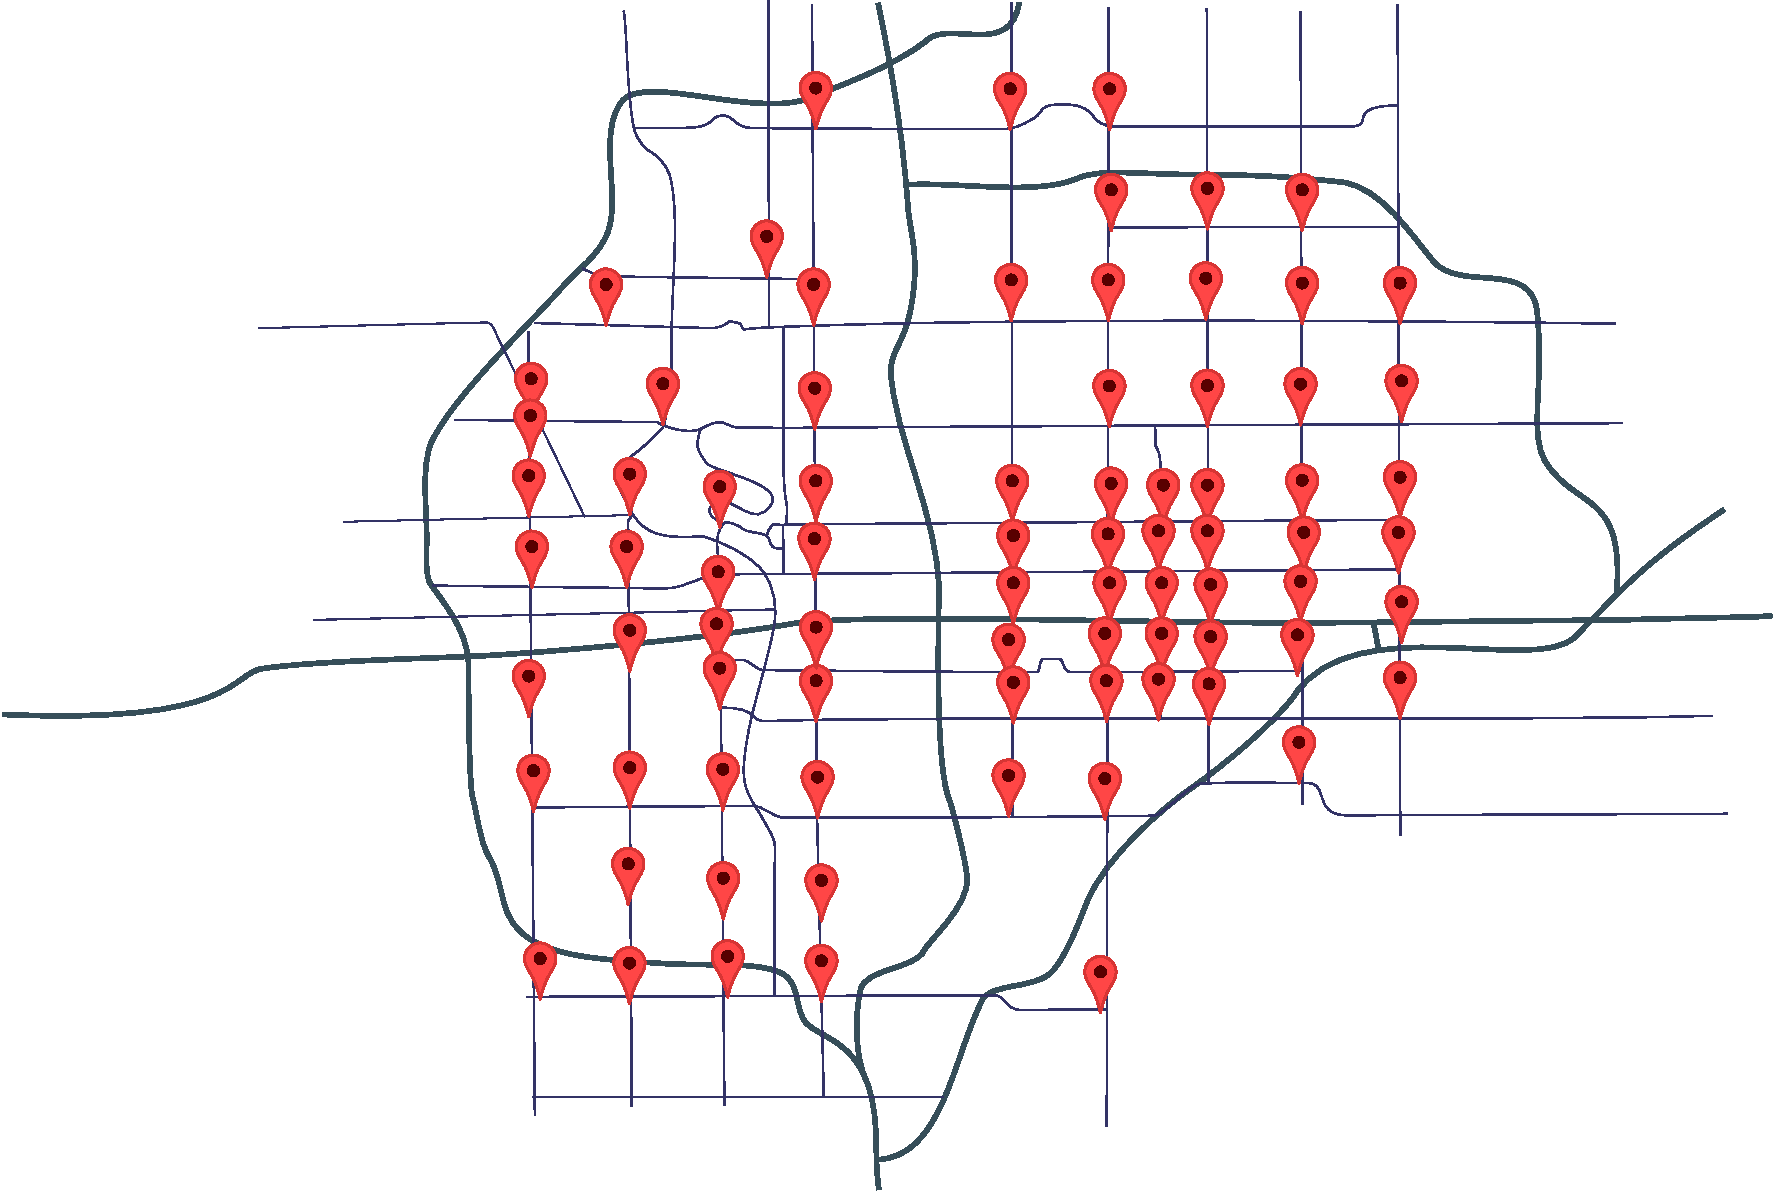
\includegraphics[width=\columnwidth]{meetup_locations_map.pdf}
	\caption{Possible public meetup locations $l_{C,q}$ for a local currency}
	\label{fig:map}
\end{figure}

Then the initiators need to perform a trusted setup ceremony with 3-12 participants. An encointer local currency should only be trusted if it was bootstrapped with a public trusted setup ceremony. In the best case you find locally renowned people to participate in the first ceremony. For the trusted setup it is recommended that public keys used for the ceremony are made public by their owners.

The currency's identifyer $C_k$ is the group public key of all registered trusted setup participants.

\subsection{Urban Scalability}
The most densely inhabitated city currently is Manila with $43'000/km^2$ \cite{manila18}. With a limit of 10 people per meetup and a participation of 100\% , $4300$ meetups would take place per $km^2$. Each meetup would be allowed an area of $232 m^2$ and the distance between meetup locations would be $r_{s,i} \approx 15m$. 
%The time window $\delta_T{s,i}$ would be as low as $180ms$, which is achievable by automated witnessing over i.e. bluetooth.

\section{Unique PoP Ceremonies}
Key signing ceremonies will be scheduled every 41 days. The interval of 41 days is an arbitrary design choice. In order for many people to be able to participate, it should be at different weekdays every time and it shouldn't happen too often - but often enough that missing one ceremony doesn't hurt too much. 
All meetups will happen at high sun $T_{C,i}$ at the same date all over the world. This is crucial because we want nobody to be able to attent two meetups for the same ceremony, because this would allow a single person to maintain more than one UPoP identity and collect a UBI in more than one currency (a Sybil attack).

\subsection{Registration}\label{ceremonyprep}
At least 24h before the start of a ceremony, participant $a$ creates a registration transaction for ceremony $i$ containing
\begin{description}
\item [$K_{a,i}^{pub}$] one-time public key
\item [$S_{C,a,j,m}$] (\emph{optional}) a proof that $a$ attended a meetup $m$ at a past ceremony $j$ successfully for the same currency $C$ (reputation).
\item [$C_k$] The local currency's identifier
\end{description}

The registration data is transferred and stored confidentially to mitigate \emph{linkability} accross ceremonies.
\subsection{Assignment}

For each local currency $C_k$, the system then assigns people from the set of registered participants $A_{C,i}$ to meetups $m_{C,i,x}$ at meetup locations from $L_C$ 24h prior the ceremony. 

In order to mitigate collusion, the assignment algorithm will apply the following rules: 

\begin{erule}\label{rule:notseeagain}
Minimize the number of participants that have met at their last ceremony already.
\end{erule}

\begin{erule}\label{rule:meetupsize}
Maximize the number of participants per meetup $N_m$ subject to $3 \leq N_m \leq 12\  \forall m$. 
\end{erule}

\begin{erule}\label{rule:noreplimit}
No meetup may be assigned with more than 1/4 of participants without reputation.
\end{erule}
	
\begin{erule}
Randomize meetup locations $l_m$ based on private randomness obtained from a TEE's secure random source.
\end{erule}

The lower limit to meetup size of 3 participants shall provide some safety (see \ref{safetythreat}). 
The upper limit of 12 attendees shall make sure that meetups can be taken out within short time and to allow each participant to remember who she/he has already signed keys with.

Rule \ref{rule:noreplimit} directly impacts the maximum adoption rate: A population of 1M will take at least $\frac{\log(\frac{1M}{12})}{log(\frac{4}{3})} \approx 40$ ceremonies to build up.

\subsubsection{Computational Complexity}
Rules \ref{rule:notseeagain}, \ref{rule:meetupsize} and \ref{rule:noreplimit} form an np-hard optimization problem. Therefore, the assignment has to be performed off-chain.

\subsection{Meetup Procedure}
Shortly before high sun $T_{C,i}$, each attendee $a_n$ shows up at the assigned location $l_m$ and votes on the number of physically present participants $\nu_{m,n}$ using the \encointer mobile phone app. The participant then broadcasts a \emph{claim of attendance} 

\begin{equation}
\zeta_{m,n} = \left(K_{a,i}^{pub}, i, m, \nu_{m,n} \right)
\end{equation}

\begin{erule}
	$\zeta_{m,n}$ has to be broadcast to all meetup participants within $\Delta t_C$ after $T_i$, as attested by the receivers. No latecomers shall be attested.
\end{erule}

\begin{equation}
\Delta t_C = \frac{min\left(dist\left(l_{C,i}, l_{C,k}\right)\right)}{v_{max}} \forall l_{C,k} \in L_C \setminus l_{C,i} 
\end{equation}

Where $v_{max} = 300km/h$ is an \encointer parameter chosen to make it impractical to attend two adjacent ceremonies.

Following the mutual broadcast of claims, participants then attest the physical presence of all counterparties by pairwise signing each others claims. More precisely, participant $a_r$ returns an attestation $\mathcal{A}_r\left(\zeta_{m,n}\right)$, signed with her private key $K^{priv}_{r,i}$ to participant $a_n$ and vice-versa.

\subsection{Witnessing Phase}
During the \emph{witnessing} phase $T_{C,i}\ until\ T_{C,i} + 24h$, each attendee sends his/her collected attestations to the \encointer chain for validation. The system then registers attestations and individual votes $\nu_n$ subject to a set of rules:

\begin{erule}
	Only consider attestations from \emph{other} participants \emph{assigned to the same meetup $m$} and the same ceremony $i$.
\end{erule}

\subsubsection{Storage Complexity}
The \emph{witnessing} registry has a storage complexity of $O(m*n^2)$ where m is the number of meetups and n the number of participants per meetup.

\subsection{Validation}
At the end of the \emph{witnessing} phase, the system validates all meetups subject to the following rules: 

Let $\mathcal{\bar M}_m$ be the set of participants for meetup $m$ with at least one valid attestation from another member in $\mathcal{\bar M}_m$.

Let $\mathcal{\hat M}_m$ be the set of participants for meetup $m$ with reputation (wo can prove recent attendance with $S_{C,a,j,x} |i-j<2$) and at least one valid attestation for meetup $m$ from another member in $\mathcal{\hat M}_m$.

Let $\hat\nu_m$ be the majority vote among $\mathcal{\hat M}_m$.

\begin{erule}\label{rule:votingcorrectly}
	Only consider participants $a_n \in \mathcal{\bar M}_m$ whose vote $\nu_n = \hat\nu_m$
\end{erule}

\begin{erule}
	Only consider participants who collected at least $|\mathcal{\hat M}_m|-2$ attestations.
\end{erule}
\begin{erule}\label{rule:hasattested}
	Only consider participants $a_n \in \mathcal{\bar M}_m$ who have attested $|\mathcal{\hat M}_m|-2 \leq N_n \leq \hat\nu_m$ participants.
\end{erule}

\subsubsection{Computational Complexity}
Validation has a complexity of $O(m*n^2)$ where m is the number of meetups and n the number of participants per meetup. 

\subsection{Reward}
All participants who passed the validation above are issued an amount of $\mathcal{R}_C$ as a universal basic income. $\mathcal{R}_C$ can be defined and adjusted per local currency by means of on-chain governance.  

\subsection{Unique Proof-of-Personhood}
Attending one meetup supplies the individual with a simple proof-of-personhood (PoP). However, it doesn't prove that one individual maintains exactly one PoP over time. The more subsequent ceremonies an individual attends, the more trustworthy is his/her Unique-PoP (UPoP) claim with respect to uniqueness.

\subsection{Threat Model}
The \encointer UPoP protocol needs to defend against two categories of adversaries:
\begin{itemize}
	\item those who try to get more than one reward per ceremony (sybil attack)
	\item those who try to sabotage the \encointer ecosystem even if this comes at a cost.
\end{itemize}
Both categories will collude among themselves to achieve their goal.

\begin{hypothesis}\label{hypothesis:secureifmajorityhonest}
	The \encointer UPoP Protocol is secure if a majority of participants with reputation for each ceremony and each meetup is honest and successfully registers their non-empty attested claims to the blockchain in time. 
\end{hypothesis}

Above hypothesis as not formally proved here. We expect to get probabilistic security with regard to the following attacks:

\subsubsection{Illegit Videoconference}
People may try to meet virtually instead of physically. \emph{Mitigated subject to Hypothesis \ref{hypothesis:secureifmajorityhonest}}
\subsubsection{Surrogates}
An adversary might pay other people to attend ceremonies on behalf of identities controlled by the adversary. The effect is similar to people renting out their identity. \emph{This attack is out of scope as it doesn't affect issuance.}
\subsubsection{Oversigning / Social Engineering}
Attendees might talk others into signing more than one pseudonym per person. Bribery could happen too. \emph{Mitigated by rules \ref{rule:votingcorrectly} and \ref{rule:hasattested} subject to Hypothesis \ref{hypothesis:secureifmajorityhonest}}
\subsubsection{Systematic No-Show}
a meeting might become invalid if too many participants don't show up (deliberately). \emph{Mitigated subject to Hypothesis \ref{hypothesis:secureifmajorityhonest}} 
\subsubsection{Flooding}
An adversary could register large numbers of fake participants who will never show up. This could prevent legit persons to participate.
 \textit{Mitigated by rule \ref{rule:noreplimit}}.
\subsubsection{Threats to Personal Safety}\label{safetythreat}
As ceremony members need to meet in person, all risks involved with human encounters apply. These risks are reduced by randomizing participants and by the minimal group size of 3 persons. Participants are advised to choose public places for ceremonies.
Threats by non-participants who want to hurt the \encointer ecosystem by attacking participants are mitigated if group $s$ keeps their exact meeting point private. 

%%%%%%%%%%%%%%%%%%%%%%%%%%%%%%%%%%%%%%%%%%%%%%%
\section{Monetary Policy}
Unlike Bitcoin, \encointer local currencies don't have a hard-capped supply. The more people are joining the ecosystem, the more money is issued. Every PoP-ceremony participant will receive one reward per attended ceremony as an unconditional basic income (UBI). 
%The value of one unit is therefore connected to the willingness of people to spend time to attend key signing parties. Beyond issuance, the possibility of obtaining a digital identity might be especially beneficial in developing countries where people might own a mobile phone but not a state-issued ID. 

To analyze the macroeconomics of such a basic income scheme let's look at the steady state of a stationary economy with a fixed population and no economic growth. 

If we'd just issue a fixed reward after every ceremony, constant absolute nominal inflation would result. The real value of one (constant) reward would decrease over time and our UBI would become meaningless. If we want our UBI to maintain meaningful value, we can either introduce increasing rewards which may be negatively percieved as hyperinflation. Or we introduce a demurrage fee, constantly ''burning'' money. Demurrage has been tested with local currencies \cite{WIR}, \cite{Chiemgauer} and the cryptocurrency Freicoin \cite{freicoin}. \encointer will employ demurrage as a nominally deflationary measure to compensate for the inflation due to ceremonies. This way, a parametrizable percentage of the money supply will be frequently redistributed in egalitarian fashion. The demurrage fee can thus be understood as a tax to the ''decentralized state'' that performs the redistribution of wealth.

Fig \ref{fig:ubi-demurrage} shows our example economy reaching an equilibrium state. For an example demurrage of 7\% per month, the money supply saturates at around 100'000 tokens. Such a demurrage causes a deliberate incentive to spend as quickly as possible instead of saving. A high money velocity can be expected. For simplicity, we assume a money velocity of one per ceremony (the sum of money changing hands between two subsequent ceremonies equals the total money supply). With a stable money supply around 100'000 tokens the total of our ceremony rewards (10'000 tokens) will maintain a constant real value of 10\% of all the spending during one period. That ratio will decrease with decreasing rates of demurrage.

Real economies are not stationary and it is not obvious, what a good amount of UBI would be. \encointer therefore allows local currencies to choose their parameters freely by means of on-chain governance. 

\begin{figure}
	\centering
	\def\svgwidth{\columnwidth}
	\input{ubi-vs-demurrage-balance.pdf_tex}
	\caption{Money supply for a stationary economy with a demurrage fee of 7\% per month and a population of 10'000 participants. After an initial phase, the UBI of 1 token per ceremony maintains a constant ratio to the total money supply and therefore maintains a constant real value.}
	\label{fig:ubi-demurrage}
\end{figure}

%Exponential community growth causes exponential growth of money supply. If community participation should one day saturate, money issuance will be constant and relative inflation rate will therefore decrease over time as shown in figure \ref{fig:inflation}.

%With such a policy in place, no early adopter should expect to get rich by hoarding as adoption drives inflation and demurrage will further disincentivize saving. 

One must expect that people with idle currency will try to avoid demurrage and buy assets better suited to store value, thereby reducing the real value of the \encointer currency. A nation state can enforce a legal tender and force citizens to pay taxes in national currency. An \encointer communitiy on the other hand could promote the use of its currency by social pressure. 

Another way of applying this technology would be to use \encointer tokens as trusted vouchers for cash transfer schemes in fiat currency, run by a state or by NGOs. In this case demurrage should be disabled and replaced by verifiably burning tokens upon exanging them for fiat.

%%%%%%%%%%%%%%%%%%%%%%%%%%%%%%%%%%%%%%%%%%%%%%%%%%%%%%%%%
\section{dPoET Consensus}
The major technical innovation of Bitcoin is its use of PoW to avoid double spends in a decentralized digital cash scheme. The higher the cost of a double spend attack, the more secure the Bitcoin blockchain.
The security of Bitcoin relies on mining power. Miners invest in infrastructure and energy as long as this remains profitable. Mining power therefore depends on the real value of miner income being proportional to Bitcoin exchange rate. 

PoS blockchain security on the other hand relies on game theory. Gaining control over the majority of stake to attack a PoS chain would destroy the real value of that stake, hurting the attacker most. PoS blockchain security therefore is proportional to its total market capitalization. A yet unsolved issue with PoS is the \textit{nothing-at-stake} dilemma \cite{poelstra15} which may cause uncontrollable forks.

PoET has similar security properties like PoW as it is just an energy-efficient replacement for PoW to elect the validator who may write the next block to the blockchain. Each validator TEE samples a uniform random number $u \in [0..1)$ and waits for an exponentially distributed wait time defined by:
\begin{equation}
	t = -\frac{ln(1-u)}{\lambda}
\end{equation}
$\lambda$ has to be adjusted to validator population size to reach a defined average block time, similar to Bitcoin's difficulty adjustment.

Everyone with a supported TEE hardware can join the validator set and gets equal probability of being selected to generate the next block. 
Therefore, the 51\% (double spend) attack applies to PoET as well. The difference is just that it's not 51\% of PoW mining power but 51\% of TEE devices in the network.   

POET by itself is not secure because an attacker might spawn the same enclave multiple times on a single TEE in parallel. A mitigation for such a \emph{replay attack} has been proposed in \cite{rote}.

\encointer makes such an attack very expensive by demanding that every validator must be linked to a unique person. Every person maintaining her PoP may run at most one validator.

Each \encointer validator node waits a random time before generating a new block according to PoET. It then assembles transactions into a block including a PoET and broadcasts the block to the network. 

In bitcoin, all nodes believe in the blockchain accumulating the most PoW since genesis. In \encointer, nodes believe in the blockchain accumulating the highest PoET difficulty $\sum_i \frac{1}{\lambda_i}$. We call this consensus algorithm \textit{democratic proof of elapsed time} (dPoET)
\subsection{Settlement Finality}
Like PoW, dPoET only delivers probabilistic transaction finality.

\section{Trusted Execution Environment Security}
TEEs aim to provide the necessary guarantees for secure remote computation. They should provide integrity and confidentiality guarantees when executing software on a computer maintained by an untrusted party. The most recent TEEs rely on software attestation, a process that guarantees the user that she's communicating with a known piece of code running inside a secure container on a genuine trusted hardware by means of a manufacturer signature.

As criticized in \cite{costan16}, manufacturers seem to follow a security by obscurity principle not disclosing design internals necessary for a proper security review. Their \textit{in dubio contra reum} analysis of Intel SGX shows vulnerabilities to cache timing and sidechannel attacks. \textit{Foreshadow} \cite{foreshadow} falsified confidentiality as well as integrity claims for SGX but the attack is mitigated for now. ARM TrustZone on the other hand is only an IP core and design details are left to the manufacturer, equally reluctant to disclose details. 

Since at least the post-Snowden era, one also has to be concerned about manufacturers being forced by their state to introduce deliberate backdoors. Even if open-source TEEs like Keystone \cite{keystone} might soon deliver devices, one would still have to trust the manufacturer not to tamper with the design. 
%ethereum VDF ASIC: https://electronics.stackexchange.com/questions/391976/exotic-semiconductors-for-fast-digital-asic/392359

While all this is disturbing, it should be put in perspective. Information security is a never-ending race. All blockchain solutions are software running by large part on Intel CPUs. While hardware wallets may give us some comfort concerning our funds private keys, there's no guarantee on confidentiality when considering sidechannel attacks. 

The \encointer cooperative will follow developments closely and maintain an up to date list of accepted TEE manufacturers' attestation keys. Even if the author is not satisfied with today's TEEs security guarantees, he considers the ecological downsides of PoW to be much more severe for society as a whole and therefore proposes to make heavy use of TEEs for \encointer.

\section{Proportional Transaction Fees}
Bitcoin transactions may pay a fee to the miner including the transaction in his block. Because Bitcoin has a hard cap on block size, a market develops for fees and miners choose the best-paying transactions to fill a block. This effect prevents micropayments effectively undermining adoption in developing countries. While IOTA \cite{iota} and Nano \cite{nano} have zero transaction fees they must use a small PoW as a measure against spam transactions. Even though small, PoW limits the possibilities to use mobile or IoT devices to send transactions.

\encointer suggests yet another way: Each transaction must include a PoET of 0.5 seconds as an anti-spam measure. This PoET can be delegated to any remote-attested TEE. Nowadays, even mobile devices feature a TEE and would therefore be able to provide a PoET. However, there is no manufacturer yet who provides remote attestation for these mobile phone TEEs. This may be possible in the future. Requiring a TEE to send transactions comes with a nice side benefit: The TEE can be used as a hardware wallet for private keys, effectively mitigating the weakest link in blockchain security by solving the safekeeping of private keys for hot wallets.
 
Still, validator nodes need an incentive for \encointer to benefit from a large decentralized network of validators. In the spirit of the Tobin Tax \cite{tobin72} it seems beneficial to the \encointer ecosystem to charge a proportional transaction fee in the order of 0.1\% to incentivize validator nodes to process transactions. In the presence of indirect block size limitations like TEE memory size, a proportional fee may still inhibit micropayments as validators might select high-value transactions with priority. That is left to be solved when we get there.
 
\encointer targets a balance of power among multiple TEE vendors as it is unlikely that different vendors collude or show the same vulnerabilities. Such a balance of power must be incentivized in order to take place. One possible incentive would be to burn a fraction of tx fees that is proportional to the network share of the validor's TEE vendor. Minority TEEs would earn more fees than majority TEEs.

\section{Private Transactions}\label{sec:privtx}
\begin{figure}
	\centering
	\def\svgwidth{\columnwidth}
	\input{block_generation.pdf_tex}
	\caption{simplified private transaction scheme}
	\label{fig:blockgen}
\end{figure}
%Private transactions in \encointer are based on the idea of Hyperledger Sawtooth's \textit{Private Data Objects} \cite{sawtoothpdo}. 
Fig \ref{fig:blockgen} shows how transactions are processed in encrypted form. Alice creates a transaction to Bob and encrypts it with the shared verifier key $K_V^{pub}$. She then appends a PoET $P_{ET}$ and sends the tx to the network. If her device has no TEE, she can delegate the PoET to any third party, whereby she only shares the encrypted tx with the PoET provider.

The validator retrieves the most recent $state_{t-1}$ (i.e. from IPFS \cite{ipfs}), assembles transactions from its mempool and sends everything to its TEE. The TEE is able to decrypt the data to process the clearing. It then writes hashes of a transaction to the new block together with the hash of the encrypted new $state_t$ and a signature, proving which validator created the block.
The new block only contains hashes, so no private information is leaking.

In order for Bob to know he received funds, Alice sends him the plaintext $tx_A$ over a private messaging channel. Bob can then hash it and scan the blockchain for $h(tx_A)$. Both Alice and Bob then must make sure to store $tx_A$ securely and redundantly as they can't retrieve their wallet balance by scanning the blockchain. 

\subsection{Enclave Provisioning}
The shared symmetric state encryption key $K_S$ and asymmetric transaction submission key $K_V^{priv}$ is known to all registered validators. Whenever the validator set changes, a new key $K_V^{priv}$ has to be established among all validators' enclaves who can then derive $K_S$. A distributed key generation scheme like \cite{gennaro1999} or \cite{tseng2005} or shall be applied for that purpose.
The shared key is expected to change frequently, thereby improving forward-secrecy in the case of side-channel attacks.

Registering a new enclave for chain validation includes the following steps:
\begin{enumerate}
	\item initialize \encointer enclave
	\item perform remote attestation with a trusted attestation service (registered on the \encointer chain)
	\item commit attestation service quote to \encointer chain
	\item all existing validators see that the validator set changed. They validate the quote and take out a new distributed key generation.
\end{enumerate}

% nice try, but % paillier uses 10x more state size (800B instead of 96B per account)
%
%\subsection{Reducing the Impact of TEE Vulnerabilities}
%Should the state encryption key $K_S$ leak because of a vulnerability of one of the validating TEEs, all account balances could be revealed. In order to mitigate this risk, we suggest to encrypt all balances with per-account shielding keys $K_{SH}^{priv}$ and to leverage Paillier's homomorphic addition: In extension to the protocol described in \ref{sec:privtx}, the sender of a transaction has to provide the private shielding key $K_{SH}^{priv}$ to the validator in order to decrypt the origin balance, verify sufficient funds, subtract the tx value and re-encrypt the resulting balance. The shielding key of the receiver doesn't need to be known to the validator TEE as homomorphic addition can be applied for the receiver and no checks on the value are necessary if we can guarantee there will never be an overflow. While the described balance shielding reduces the risk of information leakage, it can only guarantee account balance confidentiality as long as no transactions are sent to the network after the first vulnerability exploit.

%\subsection{balance attestation}
%For taxation purposes or anti money laundering, it can make sense to disclose balances selectively. A user should be able to get a balance attestation on request. Such  

\section{Private Off-Chain Smart Contracts}
The concept of private transactions explained above can be extended to allow private calls of generic stateful smart contracts. 

%If allowing turing-complete smart contracts, we need to solve the \textit{halting problem} or the system will be vulnerable to endless loops. Ethereum uses \textit{gas} to put a price tag on each smart contract instruction executed. Execution stops deterministically when the gas budget is exhausted. 

\encointer separates transaction validation consensus from smart contract execution. Unlike Ethereum, \encointer doesn't need to execute a smart contract on every validator machine. Thanks to TEEs, it would be sufficient to run smart contracts on one TEE only, as correct execution is guaranteed. For resilience, it is of course desirable to have more than one contract TEE.

\encointer Dapps provide their own TEE infrastructure in order to provide their services. This way, they're responsible for termination properties of their contracts without any impact on the \encointer main chain. Metered execution like \textit{gas} is not necessary, opening up a new range of possibilites. 

Fig \ref{fig:calls} shows how \encointer transactions allow for an optional payload $\Lambda$ which gets included in a call table $calls_t$. \encointer hereby provides a sequential ordering of smart contract calls and all the information needed to process the call is included in $calls_t$, as shown in Fig. \ref{fig:callstable}.

It is up to the Dapp to provide TEEs with their contract key $K_C$. Dapp users should make sure the contract code is open source and $K_C$ is a manufacturer-attested TEE output.
Dapps can be stateful and their hashed state can be anchored in \encointer chain by including a $K_C$ signed transaction $tx_{C,t}$ to itself. $tx_{C,t}$ should be published in cleartext so anyone can verify execution.

Related concepts were presented by \cite{ekiden}, \cite{sawtoothpdo}

%Dapps can be understood as sidechains with their TEEs getting permissioned by the \encointer main chain. A Dapp has to register its TEEs as trusted contract executors (TCE) by means of a special \encointer transaction. Each Dapp gets assigned its own key pair $K_{dapp}$, stored in the \encointer state. Any TEE may request to join as a TCE by proving manufacturer attestation and dapp code checksum. Dapps can send and receive \encointer funds, $K_{dapp}$ beeing their wallet key.

\begin{figure}
	\centering
	\def\svgwidth{\columnwidth}
	\input{smart_contract_calls.pdf_tex}
	\caption{simplified smart contract call scheme}
	\label{fig:calls}
\end{figure}

\begin{figure}
	\centering
	\def\svgwidth{\columnwidth}
	\input{calls_structure.pdf_tex}
	\caption{calls table structure}
	\label{fig:callstable}
\end{figure}

%can execution time be longer than block time? yes.

%need TEE hardware abstraction like Asylo or ***

\section{\encointer Association}
\encointer association is a not-for-profit association under Swiss law. Its purpose is to govern the \encointer ecosystem. It fulfills the following tasks
\begin{itemize}
	\item community bootstrapping
	\item protocol updates
	\item define tx fee
	\item maintain list of accepted TEE attestation service keys
\end{itemize}
All changes are subject to a referendum by the community.

\section{Known Limitations}
\subsection{Scalability}
The proposed \encointer protocol assumes that the entire state can fit into secure memory within a TEE. This limits the number of accounts that can be registered. 

\section{Conclusion}
A novel cryptocurrency system has been introduced in conceptual detail. Main contributions are 
\begin{itemize}
	\item A novel global egalitarian approach to monetary policy allowing for a universal basic income (UBI).
	\item A new definition of trustless pseudonym key signing parties for proof-of-personhood (PoP), incentivized by \encointer tokens. 
	\item A novel unpermissioned consensus algorithm dPoET, combining PoET with PoP to achieve decentralization of power by ecological means
	\item Private token transfers with microtransaction-friendly fees and low storage footprint.
	\item Scalable trustless private off-chain smart contracts
\end{itemize}
%%%%%%%%%%%%%%%%%%%%%%%%%%%%%%%%%%%%%%%%%%%%%%%%%%%%%%%
%%%%%%%%%%%%%%%%%%%%%%%%%%%%%%%%%%%%%%%%%%%%%%%%%%%%%%
\begin{thebibliography}{00}
\bibitem{nakamoto08} Satoshi Nakamoto. Bitcoin: A peer-to-peer electronic cash system, http://bitcoin.org/bitcoin.pdf, 2008
\bibitem{ford08} Bryan Ford. Pseudonym Parties:
An Offline Foundation for Online Accountability, 2008
\bibitem{pop} Maria Borge et al. Proof-of-Personhood: Redemocratizing Permissionless Cryptocurrencies
%\bibitem{ssi} K. Wagner, B. Némethi, E. Renieris, P. Lang, E. Brunet, E. Holst. Self-sovereign Identity: A position paper on blockchain enabled identity and the road ahead, https://www.bundesblock.de/wp-content/uploads/2018/10/ssi-paper.pdf, 2018
\bibitem{sunnyking12} Sunny King, Scott Nadal. PPCoin: Peer-to-Peer Crypto-Currency with Proof-of-Stake, 2012
\bibitem{poelstra15} Andrew Poelstra. "Distributed Consensus from Proof of Stake is Impossible"
\bibitem{poet} Hyperledger. PoET 1.0 Specification.  https://sawtooth.hyperledger.org/docs/core/releases/1.0/architecture/poet.html
\bibitem{costan16} V. Costan S. Devadas. Intel SGX Explained. Tech. rep., Cryptology ePrint
Archive, 2016.
\bibitem{foreshadow} Jo Van Bulck et.al. Foreshadow: Extracting the Keys to the Intel SGX Kingdom with Transient Out-of-Order Execution, 2018
\bibitem{trustzone} Introducing ARM TrustZone. https://developer.arm.com/technologies/trustzone
\bibitem{tobin72} J. Tobin. The New Economics One Decade Older. The Eliot Janeway Lectures on
Historical Economics in Honour of Joseph Schumpeter,
Princeton University Press, 1972
\bibitem{saberhagen14} Nicolas van Saberhagen, CryptoNote v 2.0, https://cryptonote.org/whitepaper.pdf, 2014
\bibitem{buenz18}B. Bünz, J. Bootle, D. Boneh, A. Poelstra, P. Wuille, Greg Maxwell. Bulletproofs: Short Proofs for Confidential Transactions and More,  IEEE S\&P 2018
\bibitem{bensasson14}Eli Ben-Sasson, Alessandro Chiesa, Christina Garman, Matthew Green, Ian Miers, Eran Tromer, Madars Virza, Zerocash: Decentralized Anonymous Payments from Bitcoin, proceedings of the IEEE Symposium on Security \& Privacy (Oakland) 2014, 459-474, IEEE, 2014
\bibitem{poon15}Poon, Joseph. The Bitcoin Lightning Network: Scalable Off-Chain Instant Payments, 2015
\bibitem{lind17} J. Lind, I. Eyal, P. Pietzuch, E. Gün Sirer. Teechan: Payment Channels Using Trusted Execution Environments
\bibitem{ethereum} Vitalik Buterin, Gavin Wood, Joseph Lubin. Ethereum Whitepaper, https://github.com/ethereum/wiki/wiki/White-Paper, 2014
\bibitem{quorum}JP Morgan Chase. Quorum. https://github.com/jpmorganchase/quorum
\bibitem{gdpr}Regulation (EU) 2016/679 of the European Parliament and of the Council of 27 April 2016 on the protection of natural persons with regard to the processing of personal data and on the free movement of such data, and repealing Directive 95/46/EC (General Data Protection Regulation). Official Journal of the European Union, Vol. L119 (4 May 2016), pp. 1-88
\bibitem{gdprbc}European Union Blockchain Observatory and Forum, Blockchain and the GDPR
\bibitem{sawtoothpdo}Hyperledger Sawtooth Private Data Objects. https://github.com/hyperledger-labs/private-data-objects
\bibitem{niemeyer08}Gustavo Niemeyer. Geohash. https://geohash.org
\bibitem{cantillon}Richard Cantiollon. Essai sur la Nature du Commerce en Général, 1755
\bibitem{piketty}Thomas Piketty. Capital in the Twenty-First Century, 2013
\bibitem{reid12}Fergal Reid. An Analysis of Anonymity in the Bitcoin System, Security and Privacy in Social Networks, 2012
\bibitem{iota}Serguey Popov. The Tangle, http://iotatoken.com/IOTA\_Whitepaper.pdf, 2016
\bibitem{nano}Colin LeMahieu. Nano: A Feeless Distributed Cryptocurrency
Network, 2016
\bibitem{keystone}Keystone Project, https://keystone-enclave.github.io/
\bibitem{openpower}https://openpowerfoundation.org/
\bibitem{manila18}https://en.wikipedia.org/wiki/List\_of\_cities\_by\_population\_density, sampled Nov. 2018
\bibitem{ipfs}Juan Benet. IPFS - Content Addressed, Versioned, P2P File System. 2014
\bibitem{tseng2005}Yuh-Min Tseng, A Robust Multi-Party Key Agreement Protocol Resistant to Malicious Participants, 2005
\bibitem{gennaro1999}R. Gennaro, S. Jarecki, H. Krawczyk, and T. Rabin, Secure distributed
key generation for discrete-log based cryptosystems, International
Conference on the Theory and Applications of Cryptographic Tech-
niques. Springer, 1999, pp. 295–310.
%\bibitem{paillier99}Pascal Paillier, \emph{Public-key Cryptosystems Based on Composite Degree Residuosity Classes}, In EUROCRYPT, 1999
\bibitem{ekiden}Raymond Cheng et al., Ekiden: A Platform for Confidentiality-Preserving, Trustworthy, and Performant Smart Contract Execution, arXiv:1804.05141, 2018
\bibitem{rote}Matetic et al., ROTE: Rollback Protection for Trusted Execution, 26th USENIX Security Symposium, 2017
\bibitem{WIR}Stodder, J., Complementary Credit Networks and Macro-Economic Stability: Switzerland’s Wirtschaftsring, Journal of Economic Behavior and Organization, 2009
\bibitem{Chiemgauer}Gelleri, Chiemgauer Regiomoney: Theory and Proctise of Regional Currencies, 2009
\bibitem{freicoin}Freicoin: https://freico.in
\end{thebibliography}

\end{document}
